\input qpd-bootstrap

\begin{problem}{20260726}
  \meta{name}{Holding a Block on an Incline}
  \meta{setter}{Jason Zhang, CollegeBoard}
  \meta{topic}{mechanics}
  \meta{difficulty}{3}
  \meta{tags}{mechanics, friction, inclined plane, Newton's laws}

A block of mass $m$ rests on a rough incline that makes an angle $\theta$ with the horizontal.  The coefficient of static friction between the block and the incline is $\mu$.

\begin{center}
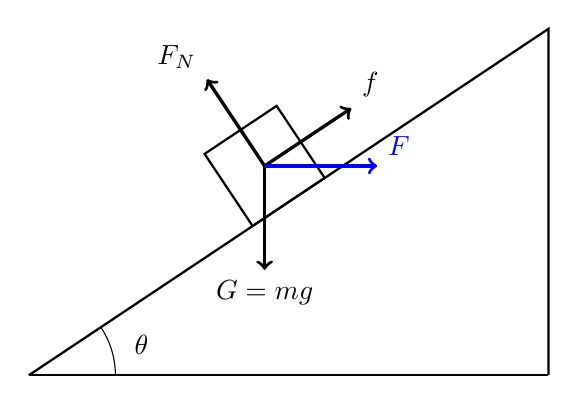
\begin{tikzpicture}[scale=1.1]
  % Incline as a right triangle, rising to the right.
  % The hypotenuse (ramp) runs from (0,0) to (6,4), slope angle ~33.7 deg.
  \draw[thick] (0,0) -- (6,0);
  \draw[thick] (0,0) -- (6,4) -- (6,0);
  % angle arc at the origin
  \draw (1.0,0) arc (0:33.7:1.0);
  \node at (1.3,0.35) {$\theta$};

  % Block centre: above the mid-slope contact point (3,2), offset half a side
  % along the ramp's outward normal (-0.555, 0.832).  The square is rotated to
  % sit flat on the ramp.
  \coordinate (B) at (2.7225, 2.416);
  \begin{scope}[shift={(B)}, rotate=33.7]
    \draw[thick] (-0.5,-0.5) rectangle (0.5,0.5);
  \end{scope}

  % Force vectors, drawn in the GLOBAL frame from the block centre B.
  % G: straight down.
  \draw[->, very thick] (B) -- ++(0,-1.2) node[below] {$G=mg$};
  % F_N: outward normal to the ramp (up-left).
  \draw[->, very thick] (B) -- ++(-0.666,1.0) node[above left] {$F_N$};
  % f: friction up the ramp (up-right along the surface).
  \draw[->, very thick] (B) -- ++(1.0,0.666) node[above right] {$f$};
  % F: applied horizontal force to the right.
  \draw[->, very thick, blue] (B) -- ++(1.3,0) node[above right] {$F$};
\end{tikzpicture}
\end{center}

An additional horizontal force $F$ is applied to the block, directed to the right.  Find the range of values of $F$ for which the block remains stationary.

\begin{assumptions}
  \item The incline is fixed; the block does not tip.
  \item Static friction can take any value between $-\mu N$ and $+\mu N$ along the incline.
  \item The applied force $F$ is horizontal, to the right (up the incline).
\end{assumptions}

\end{problem}

\begin{solution}{20260726}

The condition for the block to stay put is governed by two extrema.

\medskip
\noindent\textbf{Extremum 1: the block does not move even without $F$.}
The friction just balances the down-slope component of gravity:
\[
  f_s = mg\sin\theta,
  \qquad
  f_{s,\max} = \mu mg\cos\theta .
\]
The block is at rest without $F$ whenever $f_s \le f_{s,\max}$, i.e.
\[
  \boxed{\mu \ge \tan\theta}.
\]

\medskip
\noindent\textbf{Extremum 2: the block does not move even with $F \to \infty$.}
With $F$ applied, the normal force grows:
\[
  N = mg\cos\theta + F\sin\theta
  \;\Longrightarrow\;
  f_{s,\max} = \mu mg\cos\theta + \mu F\sin\theta .
\]
At the slip limit the up-slope force equals the friction plus the down-slope weight,
\[
  F\cos\theta - mg\sin\theta - f_s = 0
  \;\Longrightarrow\;
  f_s = F\cos\theta - mg\sin\theta \le f_{s,\max},
\]
so
\[
  F\cos\theta - mg\sin\theta \le \mu mg\cos\theta + \mu F\sin\theta
  \;\Longrightarrow\;
  \mu \ge \frac{F\cos\theta - mg\sin\theta}{mg\cos\theta + F\sin\theta}.
\]
Taking $F \to \infty$,
\[
  \lim_{F\to\infty}\frac{F\cos\theta - mg\sin\theta}{mg\cos\theta + F\sin\theta}
  = \cot\theta,
\]
so no finite $F$ can move the block when
\[
  \boxed{\tan\theta \ge \frac{1}{\mu}}.
\]

\medskip
\noindent\textbf{The range of $F$ in the three regimes.}

The two extrema partition the $(\theta,\mu)$ parameter space into three cases.  The definite formulas (when they exist) are obtained from $F_{\text{net}} = 0$ at the two slip limits.

For $F_{\min}$, friction acts up-slope at its maximum:
\[
  F\cos\theta + \mu\,(mg\cos\theta + F\sin\theta) = mg\sin\theta
  \;\Longrightarrow\;
  \boxed{F_{\min} = mg\,\frac{\sin\theta - \mu\cos\theta}{\cos\theta + \mu\sin\theta}
  = mg\,\frac{\tan\theta - \mu}{1 + \mu\tan\theta}} .
\]

For $F_{\max}$, friction acts down-slope at its maximum:
\[
  \mu\,(mg\cos\theta + F\sin\theta) = F\cos\theta - mg\sin\theta
  \;\Longrightarrow\;
  \boxed{F_{\max} = mg\,\frac{\sin\theta + \mu\cos\theta}{\cos\theta - \mu\sin\theta}
  = mg\,\frac{\tan\theta + \mu}{1 - \mu\tan\theta}} .
\]

Hence:

\begin{enumerate}
  \item If $\mu \ge \tan\theta$: the block stays put with no force, so
  \[
    \boxed{F_{\min} = 0},
    \qquad
    \boxed{F_{\max} = mg\,\frac{\tan\theta + \mu}{1 - \mu\tan\theta}} .
  \]
  \item If $\tan\theta \ge \dfrac{1}{\mu}$: no finite force moves the block, so
  \[
    \boxed{F_{\min} = mg\,\frac{\tan\theta - \mu}{1 + \mu\tan\theta}},
    \qquad
    \boxed{F_{\max} \to \infty} .
  \]
  \item If $\mu \le \tan\theta \le \dfrac{1}{\mu}$: both bounds are finite,
  \[
    \boxed{F_{\min} = mg\,\frac{\tan\theta - \mu}{1 + \mu\tan\theta}},
    \qquad
    \boxed{F_{\max} = mg\,\frac{\tan\theta + \mu}{1 - \mu\tan\theta}} .
  \]
\end{enumerate}

\end{solution}

\input qpd-end
